In this section, we introduce the change-point detection (CPD) algorithm based on subspace identification via online Dynamic Mode Decomposition (ODMD-CPD). The choice of subspace identification for CPD is motivated by the proven effectiveness of these methods in addressing complex problems (see \ref{sec:introduction}. Introduction). ODMD-CPD is applicable to non-linear, time-varying controlled systems with delays, where real-time data acquisition with irregular sampling is managed by a message queuing service. This approach is driven by real industrial challenges and grounded in the theoretical foundations discussed in Section~\ref{sec:preliminaries}. Here, we present our method coherently and provide a detailed description of the algorithm and guidelines for its application in subsequent sections.

\subsection{CPD-DMD}
As discussed in Section~\ref{sec:preliminaries}, the success of identifying a low-rank subspace over which the signal evolves, while removing noise terms, relies on selecting the appropriate rank for the subspace. Projecting data onto modes of this low-rank subspace can result in increased reconstruction error when non-conforming patterns appear in the data. Transient dynamics, in particular, cannot be adequately captured by the low-rank subspace~\citep{Kuehn2011, Gottwald2020}. Therefore, a valid selection of the subspace maximizes the reconstruction error for non-stationary signals and is crucial for its use in change-point detection~\citep{Moskvina2003}.

Long-term deployment in systems with time-varying characteristics connected to factors such as aging, wear, or environmental conditions necessitates sequential detection and updates to the subspace in a streaming manner. This allows the system to adapt to slow changes in the time series structure and to accommodate new operations that may persist for an undefined duration. The ODMD-CPD algorithm is designed to address these challenges, providing a robust and adaptive solution for change-point detection in time series data.

Firstly, when new snapshots are available, CPD-DMD updates the low-rank subspace over which the signal evolves. Secondly, the algorithm projects two stored windows of snapshot pairs, referred to as base and test matrices, onto the subspace to evaluate the reconstruction error. Finally, by comparing the reconstruction error between the base and test matrices, the algorithm computes the change-point statistics.

% \subsection{System Parameters}
\subsection{Data Stream Management}
Efficient execution of the algorithm requires preprocessing incoming data streams and managing the history of snapshots to compute the change-point statistics. Algorithm~\ref{alg:preprocessing} shows a single pass of the data preprocessing and management procedure. This procedure is executed for each available snapshot pair or in mini-batches of varying frequency and size. First, incoming snapshots are formed into time-delayed embeddings of a predefined number of delays \( h \), as shown in Eq.~\eqref{eq:hankel}. Next, the time-delayed embedding of one-step delayed snapshots \( X^\prime_{h, k: k + j} \) is compensated by control action if the control matrix \( B \) is known, or the time-delayed embedding \( X_{h, k: k + j} \) is augmented with control actions \( \Theta_{h, k: k + j} \) to form the augmented matrix \( \bar{X}_{h, k: k + j} \).

Four parameters \(a, b, c, d\) define three required snapshot sets; the base set \({\ui{\bar{X}}{B} = \{x_h(t_i)\}}^{k - b - c}_{i=k - a - b - c}\), the test set \(\ui{\bar{X}}{T} = {\{x_h(t_i)\}}^{k}_{i=k - c}\), and the learning pair \( \{\ui{\bar{X}}{L}, \ui{\bar{X}^\prime}{L}\} = {\{x_h(t_i), x_h(t_i^\prime )\}}^{k - b - c + j}_{i=k - b - c - d}\). Conveniently, storing snapshots pairs \( \{\ui{\bar{X}}{all}, \ui{\bar{X}^\prime}{all}\} = {\{x_h(t_i), x_h(t_i^\prime )\}}^{k}_{i=k - b - c - d}\) is sufficient to manage all required data efficiently. In Section~\ref{sec:guidelines}, we will explain the selection of these parameters.

% TODO: notation of number of snapshots changed from c to j
\begin{algorithm}
    \caption{Single pass of data preprocessing and management procedure}\label{alg:preprocessing}
    \begin{algorithmic}[1]
        \REQUIRE{
            \(X_{k: k + j}\), % Incoming snapshots
            \(X^\prime_{k: k + j}\), % One-step delayed snapshots
            \(\Theta_{k: k + j}\), % Control actions
            \(\ui{\bar{X}}{all}\), % Stored snapshots
            \(\ui{\bar{X}^\prime}{all}\), % Stored delayed snapshots
            \(h\), % Number of delays
            \(B\), % Control matrix
            \(a, b, c, d\) % Parameters defining snapshot sets
        }
        \ENSURE{
            \(\ui{\bar{X}}{L}\), % Learning snapshots
            \(\ui{\bar{X}^\prime}{L}\), % Learning delayed snapshots
            \(\ui{\bar{X}}{B}\), % Base snapshots
            \(\ui{\bar{X}}{T}\), % Test snapshots
            \(\ui{\bar{X}}{all}\), % Updated stored snapshots
            \(\ui{\bar{X}^\prime}{all}\), % Updated stored delayed snapshots
            \(j\) % Number of snapshots
        }

        \STATE{\(j \gets \text{number of snapshots in } X_{k: k + j}\)}

        \STATE{\(X_{h, k: k + j} \gets \text{hankelize}(X_{k: k + j}, h)\)}
        \STATE{\(X^\prime_{h, k: k + j} \gets \text{hankelize}(X^\prime_{k: k + j}, h)\)}
        \STATE{\(\Theta_{h, k: k + j} \gets \text{hankelize}(\Theta_{k: k + j}, h)\)}

        \IF{\(B\) is known}
        \STATE{\(\bar{X}_{h, k: k + j} \gets X_{h, k: k + j}\)}
        \STATE{\(\bar{X}^\prime_{h, k: k + j} \gets X^\prime_{h, k: k + j} - B \Theta_{h, k: k + j}\)}
        \COMMENT{Eq.~\eqref{eq:control-compensation}}
        \ELSE{}
        \STATE{\(\bar{X}_{h, k: k + j} \gets \begin{bmatrix} X_{h, k: k + j} \\ \Theta_{h, k: k + j} \end{bmatrix}\)}
        \COMMENT{Eq.~\eqref{eq:augmented-matrix}}
        \STATE{\(\bar{X}^\prime_{h, k: k + j} \gets X^\prime_{h, k: k + j}\)}
        \ENDIF{}

        \STATE{\(\ui{\bar{X}}{L} \gets \ui{\bar{X}}{all}(k - b - c - d: k - b - c + j)\)}
        \STATE{\(\ui{\bar{X}^\prime}{L} \gets \ui{\bar{X}^\prime}{all}(k - b - c - d: k - b - c + j)\)}

        \STATE{\(\ui{\bar{X}}{all} \gets \begin{bmatrix} \ui{\bar{X}}{all}(j: k) & \bar{X}_{h, k: k + j} \end{bmatrix}\)}
        \STATE{\(\ui{\bar{X}^\prime}{all} \gets \begin{bmatrix} \ui{\bar{X}^\prime}{all}(j: k) & \bar{X}^\prime_{h, k: k + j} \end{bmatrix}\)}

        \STATE{\(\ui{\bar{X}}{B} \gets \ui{\bar{X}}{all}(k - a - b - c: k - b - c)\)}
        \STATE{\(\ui{\bar{X}}{T} \gets \ui{\bar{X}}{all}(k - c: k)\)}
    \end{algorithmic}
\end{algorithm}


\subsection{Learning Procedure}\label{learn-cpd}
The learning procedure involves updating the Dynamic Mode Decomposition (DMD) model with new snapshots and forgetting old ones to track the system's time-varying characteristics. This procedure is outlined in Algorithm~\ref{alg:learning}.

\begin{algorithm}
    \caption{Single pass of learning procedure of CPD-DMD}\label{alg:learning}
    \begin{algorithmic}[1]
        \REQUIRE{
            \(\ui{\bar{X}}{L}\),
            \(\ui{\bar{X}^\prime}{L}\),
            \(c\),
            \(j\)
        }
        % \ENSURE{\(\Phi \)}
        \STATE{\(\tilde{c} \gets \text{number of snapshots in } \ui{\bar{X}}{L} \)}
        \STATE{\(j^\prime \gets \tilde{c} + j - c \)}
        \COMMENT{\(\tilde{c} \leq c\) smaller before fully loaded}
        \IF{\(j^\prime > 0\)}
        \STATE{\textbf{Revert:} DMD\( (
            -\ui{\bar{X}}{L}(: j^\prime),
            -\ui{\bar{X}^\prime}{L}(: j^\prime)
            ) \)}
        \COMMENT{Eq.~\eqref{eq:precision-matrix-update},~\eqref{eq:online-dmd-update}}
        \ENDIF{}
        \STATE{\textbf{Update:} DMD\( (
            \ui{\bar{X}}{L}(- j: ),
            \ui{\bar{X}^\prime}{L}(- j: )
            ) \)}
        \COMMENT{Eq.~\eqref{eq:precision-matrix-update},~\eqref{eq:online-dmd-update}}
        % \STATE{\(\Phi \leftarrow \text{DMD}()\) \COMMENT{retrieve full modes}}
    \end{algorithmic}
\end{algorithm}

Initially, we verify the number of snapshots in the learning set and revert the DMD subspace if the learning set is fully loaded. Note that the learning set might not be full at the start of the learning procedure but must contain at least \((m + l) h\) snapshots, assuming unique measurements and that the learning set \(\ui{\bar{X}}{L}\) has full column rank. Subsequently, we update the DMD subspace with new snapshots entering the learning set. This procedure is repeated for each snapshot pair available or in mini-batches, whose frequency and size may not be uniform, governed by the upstream message queuing service.

\subsection{Detection Procedure}\label{detect-cpd}
The detection procedure, executed before the learning procedure, computes the change-point statistics. This sequence is crucial to avoid false negatives, as new snapshots may represent transient dynamics, and updating the DMD subspace beforehand could result in misidentification. Although the impact of this sequence is minimal for rank-one updates since both procedures are executed in the same pass, its importance grows with the relative size of the mini-batch to the potential span of the change-point. Nevertheless, aligning with best practices prevents any information leaks.

Algorithm~\ref{alg:detection} details the detection procedure. First, we project the base and test matrices onto the DMD subspace. Second, we reconstruct the full state representation and calculate the sum of squared Euclidean distances between the data and their DMD reconstruction. Third, we normalize this sum by the number of snapshots in the matrices. Finally, we compute the change-point statistics as the ratio of errors between the test and base matrices.

In cases where the error ratio is less than 1, the reconstructed test set \(\ui{\tilde{\bar{X}}}{T}\) captures more information about \(\ui{\bar{X}}{T}\) than the reconstructed base set \(\ui{\tilde{\bar{X}}}{B}\) about \(\ui{\bar{X}}{B}\). This rare scenario typically occurs when the signal is stationary but the noise variance decreases in the test set compared to the training set. Although this phenomenon is interesting as it indicates a change in noise variance and the end of transient regime states, it is not considered in this paper, and we truncate the value to 1 and shift the score to zero, defining the minimum energy of matching errors.

\begin{algorithm}
    \caption{Single pass of detection procedure of CPD-DMD}\label{alg:detection}
    \begin{algorithmic}[1]
        \REQUIRE{
            \(\ui{\bar{X}}{B}\),  % Base matrix
            \(\ui{\bar{X}}{T}\),  % Test matrix
            \( \Phi \)            % DMD modes matrix
        }
        \ENSURE{
            \(Q_k\)  % Change-point statistics
        }
        \newline{\textbf{Project matrices onto DMD subspace}}
        \STATE{\(
            \ui{\tilde{\bar{X}}}{B} \gets \Phi^T \ui{\bar{X}}{B} \newline
            \ui{\tilde{\bar{X}}}{T} \gets \Phi^T \ui{\bar{X}}{T}
            \)}
        \newline{\textbf{Compute reconstruction errors}}
        \STATE{\(
            \ui{E}{B} \gets \sum_{i = k - a - b - c}^{k - b - c} \left \| \uis{\bar{X}}{B}{i} - \Phi \uis{\tilde{\bar{X}}}{B}{i} \right \|_F^2 \newline
            \ui{E}{T} \gets \sum_{i = k - c}^{k} \left \| \uis{\bar{X}}{T}{i} - \Phi \uis{\tilde{\bar{X}}}{T}{i} \right \|_F^2
            \)}
        \newline{\textbf{Normalize errors by the number of snapshots}}
        \STATE{\(
            \ui{E}{B} \gets \frac{\ui{E}{B}}{a} \newline
            \ui{E}{T} \gets \frac{\ui{E}{T}}{c}
            \)}
        \newline{\textbf{Compute change-point statistics}}
        \STATE{
            \(Q_k \gets \text{max}(0, \frac{\ui{E}{T}}{\ui{E}{B}} - 1)\)
        }
    \end{algorithmic}
\end{algorithm}


\subsection{Full Algorithm}
The complete change-point detection algorithm comprises three fundamental steps, as outlined in Algorithm~\ref{alg:cpd-dmd}. While the internal parameters of each step are abstracted for readability, their updates remain important. The proposed architecture is tailored for real-time execution, making it ideal for deployment in industrial environments characterized by dynamic data acquisition and irregular sampling patterns, often orchestrated by message queuing services.

\begin{algorithm}
    \caption{Single pass of CPD-DMD procedure}\label{alg:cpd-dmd}
    \begin{algorithmic}[1]
        \REQUIRE{
            \(X_{k: k + j}\),  % Current snapshots
            \(X^\prime_{k: k + j}\),  % One-step delayed snapshots
            \(\Theta_{k: k + j}\)  % Control actions
        }
        \ENSURE{
            \(Q_k\)  % Change-point statistics
        }
        \newline{\textbf{Step 1: Preprocessing the data}}
        \STATE{\(
            \ui{\bar{X}}{L}, \ui{\bar{X}^\prime}{L}, \ui{\bar{X}}{B}, \ui{\bar{X}}{T} \gets
            \text{preprocessing}( X_{k: k + j}, X^\prime_{k: k + j}, \Theta_{k: k + j})
            \)}
        \COMMENT{Refer to Algorithm~\ref{alg:preprocessing}}
        \newline{\textbf{Step 2: Detecting change-points}}
        \STATE{\(
            Q_k \gets \text{detection}( \ui{\bar{X}}{B}, \ui{\bar{X}}{T} )
            \)}
        \COMMENT{Refer to Algorithm~\ref{alg:detection}}
        \newline{\textbf{Step 3: Updating the learning model}}
        \STATE{\(
            \text{learning}( \ui{\bar{X}}{L}, \ui{\bar{X}^\prime}{L} )
            \)}
        \COMMENT{Refer to Algorithm~\ref{alg:learning}}

    \end{algorithmic}
\end{algorithm}

\subsection{Guidelines}\label{sec:guidelines}
This subsection aims to provide comprehensive guidelines for selecting hyperparameters tailored to specific use cases and problem types. Such guidance is essential for ensuring the tool's versatility across a broad spectrum of industrial applications characterized by unique conditions and specifications. By offering insights into the selection of hyperparameters, our guidelines aid the customization of the method to meet the specific requirements of different applications. To further demonstrate the impact of hyperparameter selection, we have included visual guidelines in Figure~\ref{fig:hyperparameters-all}, where all windowing parameters are changed at once, and Figure~\ref{fig:hyperparameters}, where the influence of base size, test size, and time-delays selection is shown.
\begin{figure}[H]
    \centering
    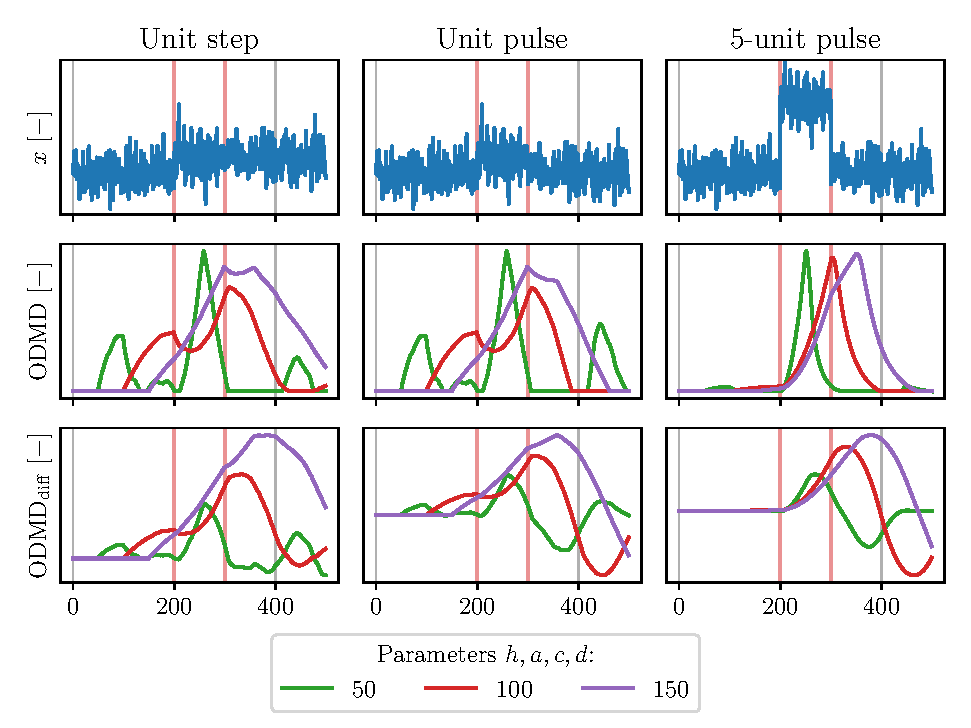
\includegraphics[width=\linewidth]{figures/parameters-influence-allatonce.pdf}
    \caption{Increasing value of all the hyperparameters at once increases robustness to noise and delays peak of CPD statistics.}\label{fig:hyperparameters-all}
\end{figure}

\begin{figure}[H]
    \centering
    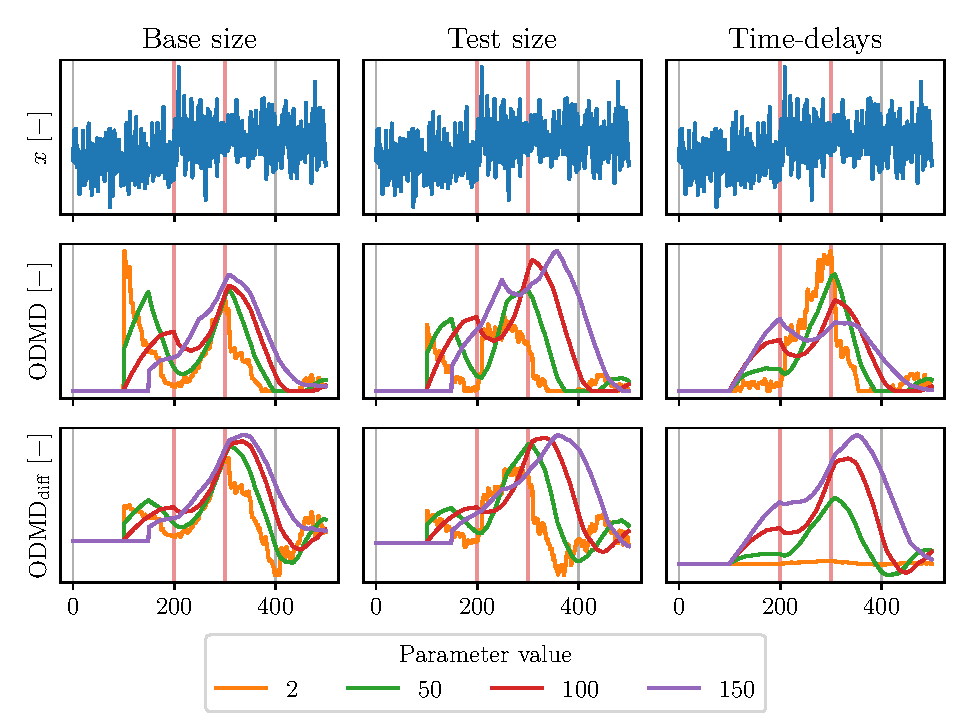
\includegraphics[width=\linewidth]{figures/Unit step-parameters-influence-ref_size_test_size_hn.pdf}
    \caption{Influence of changing hyperparameter (denoted in title of each column) values on CPD in synthetic unit step dataset.~Increasing value of base size stabilizes the score without significantly delaying the peak of CPD.~Increasing test size and number of time-delays in embedding increases robustness to noise more prominently while delying the peak of CPD.}\label{fig:hyperparameters}
\end{figure}

\subsubsection{Optimal rank}
Determining the approximate rank \( r \) of the low-rank representation of the system is a crucial and inherently subjective step in any dimensionality reduction technique. To address this challenge, we recommend employing the systematic hard-thresholding algorithm proposed by Gavish and Donoho (2014) for extracting \( r \) from noisy data. This algorithm requires information about the ratio of the number of states \((m + l) * h\) in the learning set \(\ui{\bar{X}}{L}\) and the learning window size \(a\), the selection of which is discussed later in Subsection~\ref{sec:base-window}.

Nevertheless, the proposed \( r \) may become computationally intractable for time-delayed embeddings. In such cases, we suggest using the row rank of the original data matrix \( m \) or, for augmented matrices, \( m + l \), in combination with hard-thresholding techniques to determine the optimal rank, particularly when linear system assumptions hold. For non-linear systems or situations where the collected data inadequately represent the underlying dynamics, a higher rank may be warranted to capture the dynamics effectively, while considering computational constraints and delayed response delivery. The online nature of the algorithm enables real-time adjustments to the rank, up to a certain threshold based on the significance of the \(r + 1\) singular value. These updates are facilitated by online singular value decomposition (SVD) algorithms, such as those presented in \citet{Brand2006} and \citet{Zhang2022}. For details on the implementation of rank-increasing updates, we refer readers to the original papers. Computational analysis by \citet{Zhang2019}, which applies for our proposed truncated version replacing number of states \(m\) with rank \(r\), indicates that the computational time of DMD updates scales with \( \mathcal{O}(r^2) \), with a number of floating-point multiplies of \(4n^2\), and memory requirements scale with \( \mathcal{O}(a r + 2 r ^ 2) \). This analysis can be utilized to evaluate the maximum rank for a given problem.

\subsubsection{Learning window size}
The learning window size \(d\) significantly influences the validity of the identified subspace and the accuracy of change-point detection. For identifying time-invariant systems, the learning window size should be sufficient to distinguish signal from noise and obtain the best approximation of the eigenvalues of the generating mechanism. For time-varying systems, the window size should encompass snapshots of single operating regimes or closely related operating regimes for effective learning. We propose setting the size of the base window as the lower bound on the learning window, although theoretically, the learning window could be smaller. The upper bound \(k >= b + c + d\) is determined by the number of available data points before the test window size \(c\) delayed by \(b\), as well as the size of the test window and the delay between the test and base windows. In summary, the learning window should be large enough to capture the system's dynamics without overlapping multiple operating states with distinct characteristics.

\subsubsection{Base window size and location}\label{sec:base-window}
The base window size \(a\) should reflect the expected duration of a stationary signal (single operation regime) within snapshots. This enables the reconstruction error of the base set to serve as a reference for the overall quality of the identified subspace and mitigates adverse effects on prediction accuracy. The base window should be located directly after the test window (\(b = 0\)). A value of \(a \leq d\) could prevent negative scores in collective anomalies, enabling effective differentiation between change points and collective changes.

\subsubsection{Test window size}
The test window size \(c\) determines the smoothness of change-point statistics over time. A larger test window results in smoother change-point statistics~\citep{Moskvina2003}. The selection of the test window size should consider the expected duration of the change-point, the nature of structural changes, and the desired smoothness of change-point statistics. Ideally, the peak of the statistics aligns precisely with the test window size delay from the change point. Smaller values of \(c\) decrease the delay, enhancing rapid detection but potentially missing slow drifts due to trends. Conversely, larger values of \(c\) increase stability and reduce false positives while potentially increasing false negative rates.

\subsubsection{Number of time-delays}
The number of time delays (\(h\)) is a critical parameter for ODMD-CPD in applications to non-linear systems with delayed effect of control action. Its selection relies on assumptions regarding the representativeness of snapshots with respect to the generating mechanism and the maximum expected delay of the control effect on system states. In the absence of such knowledge and with a reasonably large \(a\), \citet{Moskvina2003} recommend setting \(h = a / 2\) for the rank of the Hankel matrix. For larger \(a\), delay steps \(h_d\) may be used to capture the broadband dynamics of the system more effectively. The choice of \(h_d\) should be based on the maximum allowed number of features \((m + l)\frac{h}{h_d}\).

\subsubsection{Change-detection statistics threshold}
The threshold on change-detection statistics directly impacts the number of false positive or false negative alarms. Its proper selection further determines the delay of the detection alarm, as the rising change-point detection statistics cross the lower threshold sooner. As the CPD statistic, defined in Subsection~\ref{detect-cpd}, has no proper normalization and is influenced by the selection of other hyperparameters, the specification of constant values is challenging. As a general rule of thumb, higher recall (lower false negative rate) is achieved by setting the threshold lower. In contrast, higher precision (lower false positive rate) is achieved by setting the threshold higher. If accurate system tracking is achieved, i.e., \( r \) and \(h\) were selected so that the signal is extracted from noise well, the threshold could be set to zero while not compromising precision significantly. This may be desired in safety critical systems where higher recall helps to protect assets and life.  Generally, the threshold should be set based on the desired trade-off between precision and recall, the change point's expected duration, and the structural changes' nature.
